\chapter{Implementación de la solución}
\label{ch:stego}

A continuación, en este capítulo, vamos a ver cómo fueron los primeros usos de Stegosploit junto con los problemas derivados de éstos (\cite{stegosploit}). Más adelante pasaremos a ver qué solución propusimos para utilizar la herramienta y cómo insertamos el código malicioso en las imágenes. Por último, explicaremos cómo utilizamos FastAI con estas imágenes y qué modelos de Deep Learning acabamos usando (\cite{fastai}). %cita %cita

\section{Primeros intentos de uso de Stegosploit}
\label{sec:stego_1}

En primera instancia, leímos el paper correspondiente a la herramienta original de \textbf{Stegosploit}, y tratamos de extraer la herramienta según las indicaciones provistas por el creador de la misma.

Sin embargo, y tras seguir sus pasos, obtuvimos un error (del que hablaremos más adelante) por el que no pudimos conseguir la herramienta y que, como veremos en otro contexto, nos obligó a tener que crear un \textbf{servidor HTTP} con algunas especificaciones sobre el que ejecutar la herramienta (una vez extraída de otra manera a la que proponía el creador). Durante el desarrollo del capítulo veremos cuál fue ese error, en qué consistía, y cómo se constituyó el servidor que creamos para solucionarlo.

Para obtener la herramienta, investigamos y encontramos un repositorio de GitHub llamado \textbf{PyStegosploit} que contenía todos los útiles de la misma (\cite{pystegosploit}). De este modo, descargamos el repositorio y lo colocamos en una ubicación fácilmente accesible desde nuestro sistema de archivos.

Una vez obtenida la herramienta, ejecutamos el instrumento que propicia el encriptado de información en imágenes. Para ello nos situamos en la siguiente carpeta de la herramienta y abrimos el HTML propio de esta utilidad:

\begin{center}
\textit{PyStegosploit\textbackslash{project-stegosploit}\textbackslash{encoding}\textbackslash{iterative\_encoding.html}}
\end{center}

Si ahora ejecutamos la herramienta, nos dará el error del que hablábamos antes, y que ahora procedemos a explicar:

\subsection{Error \textit{getImageData()}}

Antes de explicar el error, vamos a poner en contexto al lector para que sepa en qué situación aparece y cómo solucionarlo.

\begin{figure}[H]
  \centering
  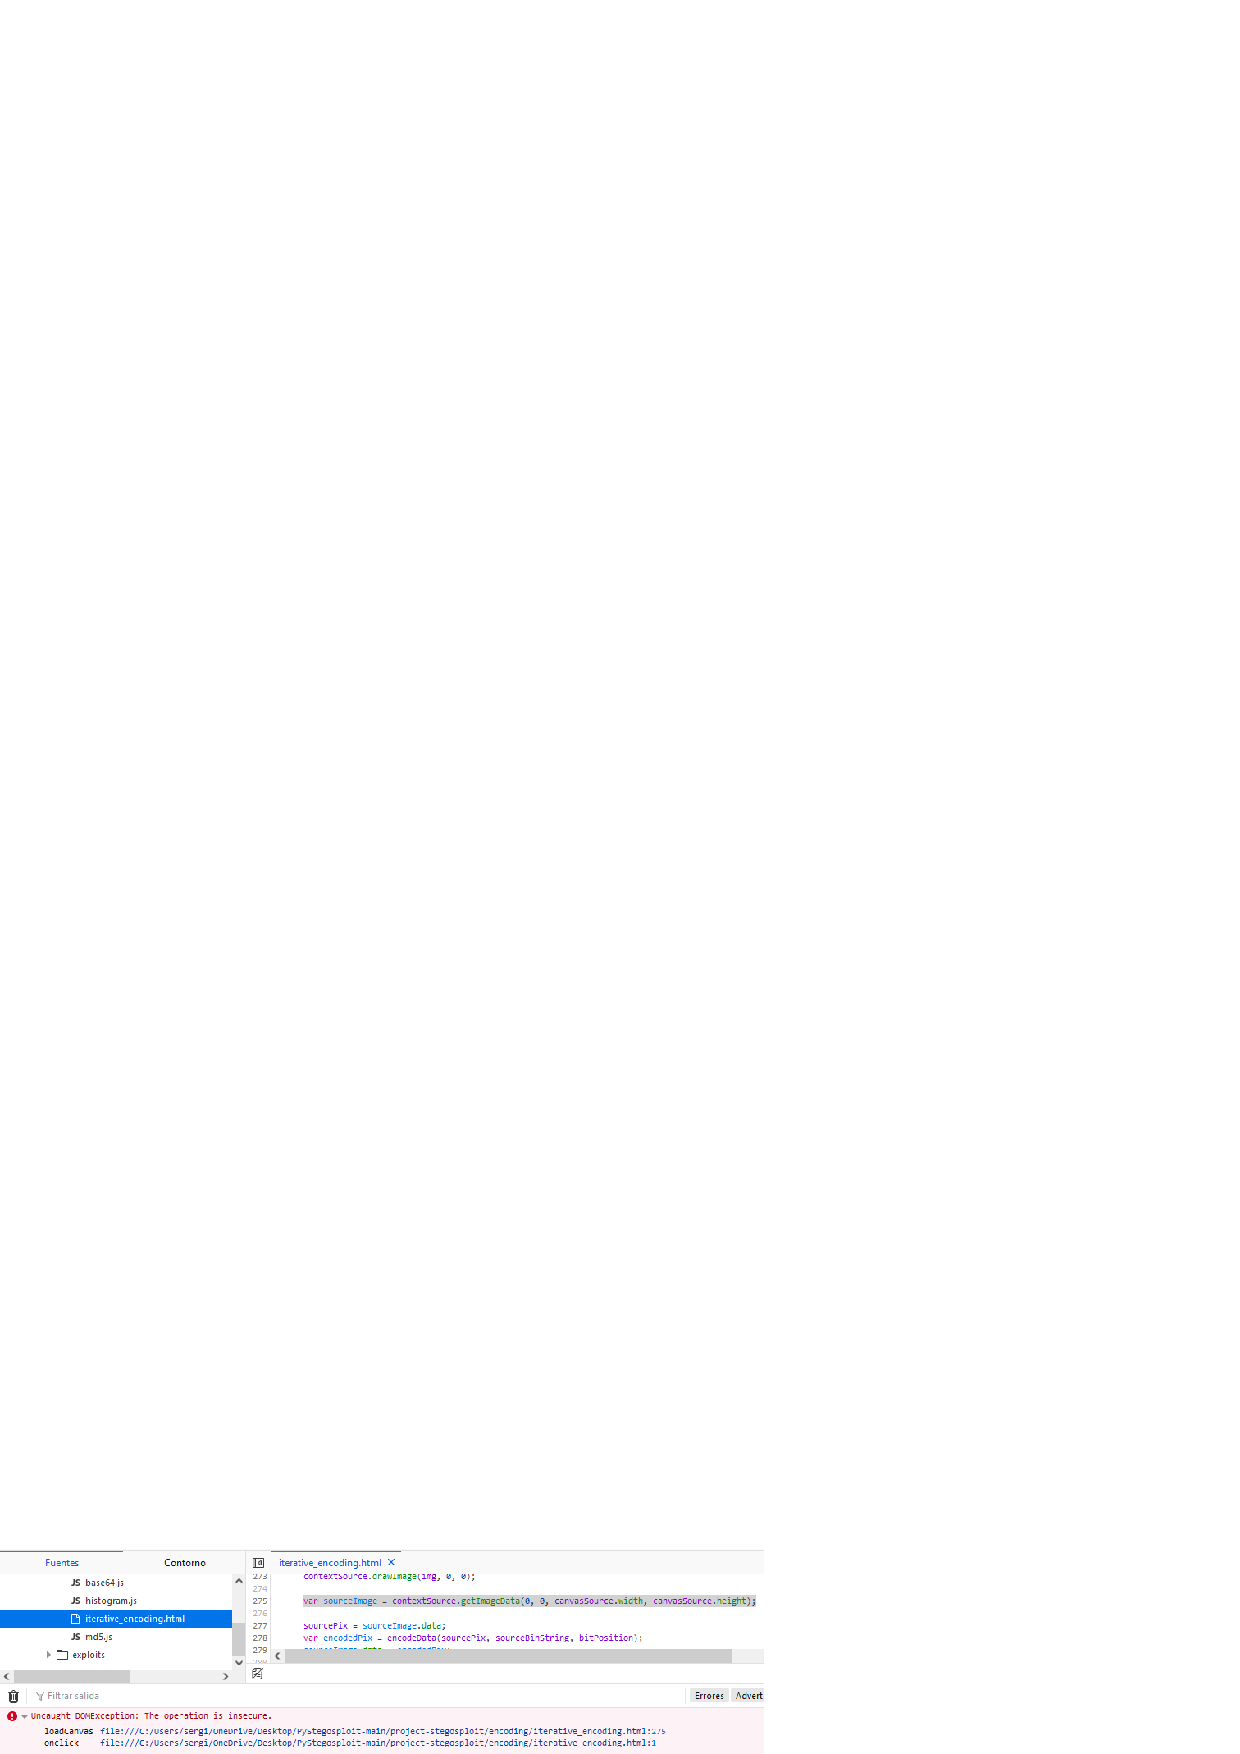
\includegraphics[width=\linewidth]{Figuras/Implementacion/getimagedata.png}
  \label{fig:getimagedata}
  \caption{Error de \textit{getImageData()}}
\end{figure}

Si ejecutamos la herramienta con una imagen del set de imágenes de COCO, y le introducimos un exploit, no funcionará. Saldrá el error que mencionamos debido a la siguiente función de Javascript: \textbf{getImageData()}.

Esta función permite obtener los datos de los píxeles de una imagen y almacenarlos en un elemento \textbf{Canvas} del HTML (\cite{getimagedata}). En principio no debería de haber ningún problema con ello, sin embargo, ocurre una cosa muy curiosa: el origen de la imagen no es \textbf{``fiable''}, y la política \ac{CORS} de la solicitud HTTP impide la ejecución de dicha función. %cita

La política \ac{CORS} es un mecanismo que usa cabeceras HTTP adicionales para que un usuario obtenga permisos para acceder a recursos determinados de un servidor desde un origen distinto a éste (\cite{CORS}). Cuando se solicita un recurso a través de una petición HTTP desde un origen distinto al que pertenece el mismo, la política entra en acción y permite, o no, el acceso a éste. %cita

Dicho esto, se entiende mejor la premisa del problema que nos atañe. Como el origen de la imagen es de otro dominio, \ac{CORS} impide la ejecución de la función \textit{getImageData()} por ser una función que interactúa con los datos de la misma.

La solución, tras investigar a conciencia, reside en añadir el siguiente atributo HTML dentro de la herramienta de encriptado de JPG de Stegosploit, concretamente en la etiqueta referente a la carga de la imagen en la página:

\begin{center}
\textit{cross-origin=``anonymous''}
\end{center}

Con el siguiente atributo se omite el intercambio de las credenciales del usuario, por lo que no debería de haber problema para poder manipular la imagen independientemente de su origen (\cite{cross-origin-anonymous}). Aun así, no es suficiente para solucionar el problema, hay que añadir una cabecera HTTP en la respuesta a la solicitud realizada por el usuario... Para ello, hay muchas utilidades y programas con los que poder hacerlo; sin embargo, lo mejor es crear un servidor HTTP desde cero que añada la cabecera HTTP. %cita

\subsection{Solución del error \textit{getImageData()}}

Antes de comenzar a explicar la creación del servidor vamos a explicar qué cabecera vamos a utilizar dentro de las peticiones HTTP, ya que sin ésta no se podría hacer nada con la herramienta.

La cabecera a añadir se denomina \textbf{Access-Control-Allow-Origin}, y es la que permite que los recursos de la respuesta HTTP puedan ser compartidos (\cite{access-control-allow-origin}). De forma resumida, un usuario realiza una petición HTTP (en nuestro caso, cargar una imagen del set de imágenes de COCO o activar la función de encriptado de la herramienta), y la respuesta de la web (modificada con el atributo \textit{cross-origin} y con la cabecera HTTP bien configurada) permitirá que la función \textit{getImageData()} y el resto de funciones que manipulen los datos de la imagen se puedan ejecutar correctamente. %cita

A continuación pasamos a explicar la creación del servidor HTTP:

\begin{figure}[H]
  \centering
  \includegraphics[width=0.60\linewidth]{Figuras/Implementacion/Server\_HTTP.png}
  \label{fig:server-http}
  \caption{Servidor HTTP}
\end{figure}

Como se puede ver en la figura, el servidor lo hemos realizado usando Python e importando las librerías necesarias para que pueda servir como un servidor local para realizar pruebas (ya que no hace falta mucho más). El servidor está diseñado para que, por cada petición HTTP que se realice por parte del usuario, se obtenga una respuesta con la cabecera HTTP de la que hablábamos; de esta forma no habrá inconvenientes para manipular los datos de las imágenes en la herramienta y, por lo tanto, el origen de las imágenes no supondrá ningún problema durante su ejecución.

Según la figura, todo parece tener el mismo aspecto que un servidor de HTTP normal y corriente; sin embargo, hay que destacar la inserción de la cabecera \textbf{Access-Control-Allow-Origin} (\cite{server-http}). La cabecera como tal puede admitir dos valores:

\begin{itemize}
\item \textbf{*}: Permite que cualquier origen pueda acceder al recurso. El acceso será permitido si el atributo \textbf{cross-origin} está definido como \textit{anonymous}.
\item \textbf{<origen>}: Permite que un origen determinado pueda acceder al recurso, pudiendo especificar sólo un origen.
\end{itemize}

Dicho esto, y como se puede apreciar en la figura \ref{fig:server-http}, usaremos el primer valor.

\subsection{Usando Stegosploit}

Si ejecutamos el servidor HTTP, lo abrimos desde el navegador, y nos posicionamos en la carpeta donde se encuentra la herramienta, podremos ejecutarla sin problemas.

\begin{figure}[H]
  \centering
  \begin{subfigure}[H]{0.30\linewidth}
  	\includegraphics[width=\linewidth]{Figuras/Implementacion/Iterative\_Encoding\_1.png}
  	\label{fig:iter-encod}
  	\caption{Encriptado de JPG}
  \end{subfigure}
  \begin{subfigure}[H]{0.45\linewidth}
  	\includegraphics[width=\linewidth]{Figuras/Implementacion/Iterative\_Encoding\_2.png}
  	\label{fig:iter-encod-2}
  	\caption{Exploit a introducir}
  \end{subfigure}
  \caption{Stegosploit}
\end{figure}

El código que hemos introducido aparece en el paper de Stegosploit y hace referencia a una vulnerabilidad que permite al atacante ejecutar código arbitrario en el contexto de los privilegios del proceso del navegador usando la corrupción de memoria. Afectaba a las versiones de Internet Explorer 8, 9 y 10 que aún no estaban parcheadas (\cite{CVE-2014-0282}). %cita

\begin{figure}[H]
  \centering
  \begin{subfigure}[H]{0.45\linewidth}
  	\includegraphics[width=\linewidth]{Figuras/Implementacion/Stegosploit\_1.png}
  	\label{fig:stegosploit-uso}
  	\caption{Primera imagen de uso del servidor}
  \end{subfigure}
  \begin{subfigure}[H]{0.45\linewidth}
  	\includegraphics[width=\linewidth]{Figuras/Implementacion/Stegosploit\_2.png}
  	\label{fig:stegosploit-uso-2}
  	\caption{Primera visualización de Stegosploit}
  \end{subfigure}
  \begin{subfigure}[H]{0.60\linewidth}
  	\includegraphics[width=\linewidth]{Figuras/Implementacion/Stegosploit\_3.png}
  	\label{fig:stegosploit-uso-3}
  	\caption{Exploit introducido}
  \end{subfigure}
  \caption{Usando Stegosploit}
\end{figure}

Como se puede ver, cuando acaba la herramienta se muestra la imagen bordeada con un marco de color rojo y con el código introducido en la imagen tras su desencriptado, para ver cómo quedaría cuando éste se realizase.

\section{Deep Learning}
\label{sec:fastai}

Ya hemos explicado la parte que más problemas nos ha dado del proyecto, ahora vamos a pasar a explicar qué herramientas y útiles de Deep Learning hemos usado para poder detectar el código introducido en las imágenes de forma eficaz.

\subsection{FastAI}

La herramienta que hemos usado para realizar este apartado tanto por sus buenas prestaciones como por la facilidad de su implementación ha sido \textbf{FastAI}. FastAI es una librería de Deep Learning que brinda de componentes de alto nivel, con los que se puede rápida y fácilmente obtener muy buenos resultados desde una base estándar de Deep Learning, es decir, sin tener que utilizar herramientas demasiado complejas para construir la estructura sobre la que se van a usar estos componentes (\cite{fastai}). %cita

Para usar FastAI, al igual que cualquier facilidad de Deep Learning, existen dos maneras:

\begin{itemize}
\item Usando una \ac{GPU}
\item Usando una \ac{CPU}
\end{itemize}

La primera de ellas es, en cuanto a rendimiento, tiempo de ejecución, y uso de recursos; bastante mejor que la segunda. Esto es debido a que una \ac{GPU} tiene, por lo general, muchos más procesadores que una \ac{CPU}, por lo tanto, el tiempo que le llevaría a una \ac{CPU} entrenar un modelo de Deep Learning podría llegar a ser incluso 10 veces más que a una \ac{GPU} (\cite{gpu-cpu}). %cita

\subsection{Google Colab}

Para este proyecto no disponíamos de una máquina con una ac{GPU} propia, de modo que hemos utilizado \textbf{Google Colab} para poder ejecutar Python desde el navegador usando una \ac{GPU} que la propia herramienta nos permite utilizar, limitada por un tiempo de uso; es decir, si excedes los recursos de procesado que se te permite utilizar, no puedes volver a utilizar la \ac{GPU} durante un tiempo (\cite{google-colab}). %cita

Mientras usamos Colab, vimos que se nos permitía hacer varias secciones de código para poder ejecutarlo alternativamente, lo cual nos ayudó a optimizar el tiempo de ejecución de la herramienta. En las siguientes figuras explicaremos qué hicimos en cada sección:

\begin{figure}[H]
  \centering
  \includegraphics[width=0.45\linewidth]{Figuras/Implementacion/Colab\_1.png}
  \label{fig:colab-1}
  \caption{Fastbook}
\end{figure}

La primera figura indica la instalación de la librería \textbf{Fastbook} de Deep Learning, utilizada específicamente en Google Colab mientras se usa FastAI en la misma herramienta. Básicamente, y de forma general, es un código que ayuda a conectar el cuaderno de Google Colab con Google Drive usando un token de autenticación (\cite{fastbook-1}, \cite{fastbook-2}). %cita %cita

\begin{figure}[H]
  \centering
  \includegraphics[width=0.45\linewidth]{Figuras/Implementacion/Colab\_2.png}
  \label{fig:colab-2}
  \caption{Montar Google Drive}
\end{figure}

La segunda figura indica que el sistema de archivos de Google Drive se va a montar en Colab. Quisimos hacerlo así ya que era la forma más rápida de obtener las imágenes alteradas con Stegosploit y las imágenes normales. Las imágenes estaban almacenadas en un archivo \textbf{.zip}.

\begin{figure}[H]
  \centering
  \includegraphics[width=0.45\linewidth]{Figuras/Implementacion/Colab\_3.png}
  \label{fig:colab-3}
  \caption{Quitar Google Drive}
\end{figure}

Este código es opcional. En nuestro caso no queríamos que los archivos de Google Drive permaneciesen en la sesión de Colab todo el rato, de modo que movimos el archivo \textbf{.zip} que contenía las imágenes a usar durante los entrenamientos de los modelos y lo pusimos en una subcarpeta de Colab que estuviera más a mano. Una vez hecho eso, ejecutamos el código de la figura y contamos así con las imágenes sin tener los archivos de Google Drive en la misma sesión.

\begin{figure}[H]
  \centering
  \includegraphics[width=0.75\linewidth]{Figuras/Implementacion/Colab\_4.png}
  \label{fig:colab-4}
  \caption{Descomprimir el \textbf{.zip}}
\end{figure}

Esta figura indica la descompresión del archivo \textbf{.zip} que contenía las imágenes a usar. De esta forma tenemos las imágenes en una carpeta y el acceso a las mismas es más sencillo.

\begin{figure}[H]
  \centering
  \includegraphics[width=\linewidth]{Figuras/Implementacion/Colab\_5.png}
  \label{fig:colab-5}
  \caption{Código para entrenar los modelos}
\end{figure}

Por último, en esta figura se muestra el código usado para entrenar los modelos, la cual vamos a pasar a explicar paso a paso:

\begin{enumerate}
\item En primer lugar, importamos el módulo \textit{visions} de la librería FastAI que contiene todos los útiles necesarios para definir un set de imágenes y entrenar un modelo para realizar tareas como la clasificación de imágenes. Seguidamente, importamos la librería \textit{torch}, necesaria para poder entrenar el modelo sobre una \ac{GPU} (\cite{pytorch}). %cita
\item A continuación, usando la siguiente instrucción, liberamos la memoria en caché sin ocupar para poder usarse en otras aplicaciones:

\begin{center}
\textit{torch.cuda.empty\_cache()}
\end{center}

En principio no es necesario utilizar esta instrucción, pero la ejecutamos igualmente por si acaso (\cite{cuda-empty-cache}).
\item Más tarde, definimos la ruta en la que se encuentran las imágenes que usaremos para entrenar los modelos, y las almacenamos en la variable \textbf{\textit{files}} con la instrucción:

\begin{center}
\textit{get\_image\_files()}
\end{center}

\item A continuación definimos una etiqueta denominada \textit{``con\_exploit''} asociada al nombre de las imágenes a las que le hemos introducido el código por esteganografía. Los nombres de las imágenes que tengan el exploit empezarán por letra minúscula, como por ejemplo \textit{imagen\_1.jpg}. De esta forma, la clasificación se centrará en los nombres de los archivos.

Al principio se basará en una clasificación por nombre, pero conforme se vaya agrandando el set de imágenes en futuros trabajos, los modelos consecuentemente irán aprendiendo bit a bit como explicábamos en anteriores capítulos, y el nombre del archivo tomará un papel secundario en la clasificación.

\item En este punto es donde definimos cómo se van a cargar los datos y con qué características y condiciones se van a presentar en los modelos. El tipo de variable que recoge esta información en Python, para este ámbito, se conoce como \textbf{DataLoader}.

En primer lugar definimos la ruta en donde se encuentran las imágenes como primer argumento de la función, seguida de la variable que almacena las imágenes y de la etiqueta \textit{``con\_exploit''} que vimos anteriormente.

El siguiente argumento es el tamaño del lote de imágenes que se van a entrenar en cada iteración. Para cada iteración se van a cotejar todas las imágenes, sin embargo, se tienen que distribuir de forma diferente en cada una para que haya una cierta aleatoriedad y que los modelos no aprendan siempre con las mismas imágenes en un mismo lote. Es decir, si queremos que el sistema prospere tenemos que forzar a que aprenda de todas las imágenes, no de sólo unas pocas que sean siempre las mismas. Esto lo conseguimos concretando este argumento.

Son 5000 imágenes, con un tamaño de lote de 20 imágenes; si dividimos obtenemos 250 lotes con 20 imágenes cada uno.

Por último, llegamos a un argumento polémico pero necesario: para que el \textbf{DataLoader} trate en condiciones las imágenes, todas ellas deben tener un mismo tamaño, lo cual es un problema ya que las imágenes tienen dimensiones muy dispares entre sí y el código introducido en unas puede suponer una gran parte de la información de la imagen. Este argumento redimensiona las imágenes para que tengan un mismo tamaño y así poder entrenarlas  en los modelos con mayor facilidad para el programa.

El problema es que al redimensionarlas se puede perder parte de la información del exploit introducido, y a pesar de que para la clasificación final pueda no afectar demasiado, al final estamos quitando datos de la imagen que podrían servir para otros casos más avanzados de detección de malware. Tras realizar varias pruebas con Stegosploit, nos percatamos que para imágenes con dimensiones menores que \textbf{500x375} píxeles no se puede introducir el exploit; por otro lado, y haciendo pruebas con Google Colab, para obtener un rendimiento óptimo de la herramienta y para que no nos diese un error por falta de memoria en la \ac{GPU}, resolvimos en establecer un tamaño de redimensionado definido en \textbf{550} píxeles (es decir, \textbf{550x550} píxeles). De esta forma evitamos la pérdida de información en su mayoría, y la herramienta de Google Colab puede funcionar sin problemas.

\item A continuación definimos una variable con la métrica que le vamos a pasar al \textit{Learner}. Un \textit{Learner} es un tipo de variable que define el modelo de Deep Learning, la métrica y el DataLoader a usar. Los hay de varios tipos, pero al tratarse de un problema de clasificación de imágenes trabajaremos con un \textit{Learner} enfocado en ese ámbito. El DataLoader ya está definido, de modo que lo pasamos como primer argumento. El modelo de Deep Learning es el segundo argumento que pasaremos, rondando entre tres posibles opciones: \textit{ResNet-34}, \textit{ResNet-18} y \textit{AlexNet}. Por último, pasaremos como argumento final la métrica que hayamos definido previamente, y que en el capítulo \ref{ch:res} explicaremos.

Los \textit{Learner} tienen más argumentos adicionales como por ejemplo la capacidad de aprendizaje del modelo, o qué porcentaje del set de imágenes irá destinado a entrenamiento y a validación... Por lo general, hemos decidido dejarlo por defecto, puesto que sus valores se ajustaban a nuestros objetivos y a nuestros recursos: \textbf{capacidad de aprendizaje de un 0,001\%, un 80\% de imágenes para entrenamiento y un 20\% para validación}.
\item Como último paso de todos vamos a poner una instrucción utilizada para refinar el modelo de Deep Learning que hemos definido en el Learner. Como único argumento le hemos puesto el número de iteraciones que queremos que haga (cada una con el set de imágenes distribuido de forma aleatoria como indicábamos anteriormente). En este caso hemos decidido poner 25, para que tenga así un rango de aprendizaje más amplio.

\end{enumerate}

En el siguiente capítulo hablaremos en detalle de las métricas utilizadas, mostraremos los resultados de los modelos y haremos una comparativa entre ellos, decidiendo cuál es el mejor y por qué.